% Created 2025-06-07 Sat 00:24
% Intended LaTeX compiler: pdflatex
\documentclass[t]{beamer}
           \usepackage[orientation=portrait,size=a0,scale=1,debug]{beamerposter}
           \usepackage[absolute,overlay]{textpos}
\usepackage{fontspec}
\usepackage{emoji}
\usepackage{xcolor}
\usepackage[language=english,backend=biber]{biblatex}

\AtEveryBibitem{%
\clearfield{issn} % Remove issn
\clearfield{doi} % Remove doi
\ifentrytype{online}{}{% Remove url except for @online
\clearfield{url}
}
}
\renewcommand*{\bibfont}{\small}
\usepackage{beamerorgposter}
\usepackage{fontspec}
\usepackage{fontenc}
\usepackage{microtype}
\usepackage{xstring}
\setlength{\emergencystretch}{2em} % Fix overflows
\usepackage{polyglossia}
\addbibresource{Publications.bib}
\author{
Marc Baaden$^{1}$
\\
\vspace{5mm}
\normalsize{$^{1}$Université Paris Cité, CNRS,}
\normalsize{Laboratoire de Biochimie Théorique,}
\normalsize{13 rue Pierre et Marie Curie, 75005, Paris, France}
}
\usetheme{default}
\useinnertheme{rectangles}
\date{\today}
\title{Interactive Molecular Simulations and Analyses for Everyone}
\hypersetup{
 pdfauthor={Marc Baaden},
 pdftitle={Interactive Molecular Simulations and Analyses for Everyone},
 pdfkeywords={},
 pdfsubject={},
 pdfcreator={Emacs 29.4 (Org mode 9.6.15)}, 
 pdflang={English}}
\begin{document}




\begin{frame}[label={sec:org8d12b2d}]{}
\begin{columns}
\begin{column}{0.27\columnwidth}
\begin{block}{\emoji{chequered-flag} Introduction}
\begin{alertblock}{The Challenge}
\begin{itemize}
\item \alert{Interactive Molecular Simulations \& Analyses} (IMSA) are powerful but underutilized
\item High technical barriers limit adoption
\item Complex installations discourage exploration
\item Limited access to specialized hardware
\end{itemize}

\vspace{5mm}

\begin{figure}[htbp]
\centering
\includegraphics[width=.9\linewidth]{../img/molplay-banner1.png}
\caption{\label{fig:orgb94cfe9}Interactive Molecular Simulation and Analysis examples.}
\end{figure}
\end{alertblock}

\begin{alertblock}{One Possible Solution: MolPlay \autocites{molplayurl}[][]{hal-04794544}}
MolPlay is a \emph{bootable USB platform} providing turnkey access to IMSA.

\vspace{5mm}

Key Features:
\begin{itemize}
\item No installation required
\item Works on standard hardware
\item User-friendly interface
\item Curated examples included
\item Portable and self-contained
\end{itemize}

\vspace*{1.8cm}
\end{alertblock}
\end{block}

\begin{block}{\emoji{magnifying-glass-tilted-right} Architecture}
\begin{figure}[htbp]
\centering
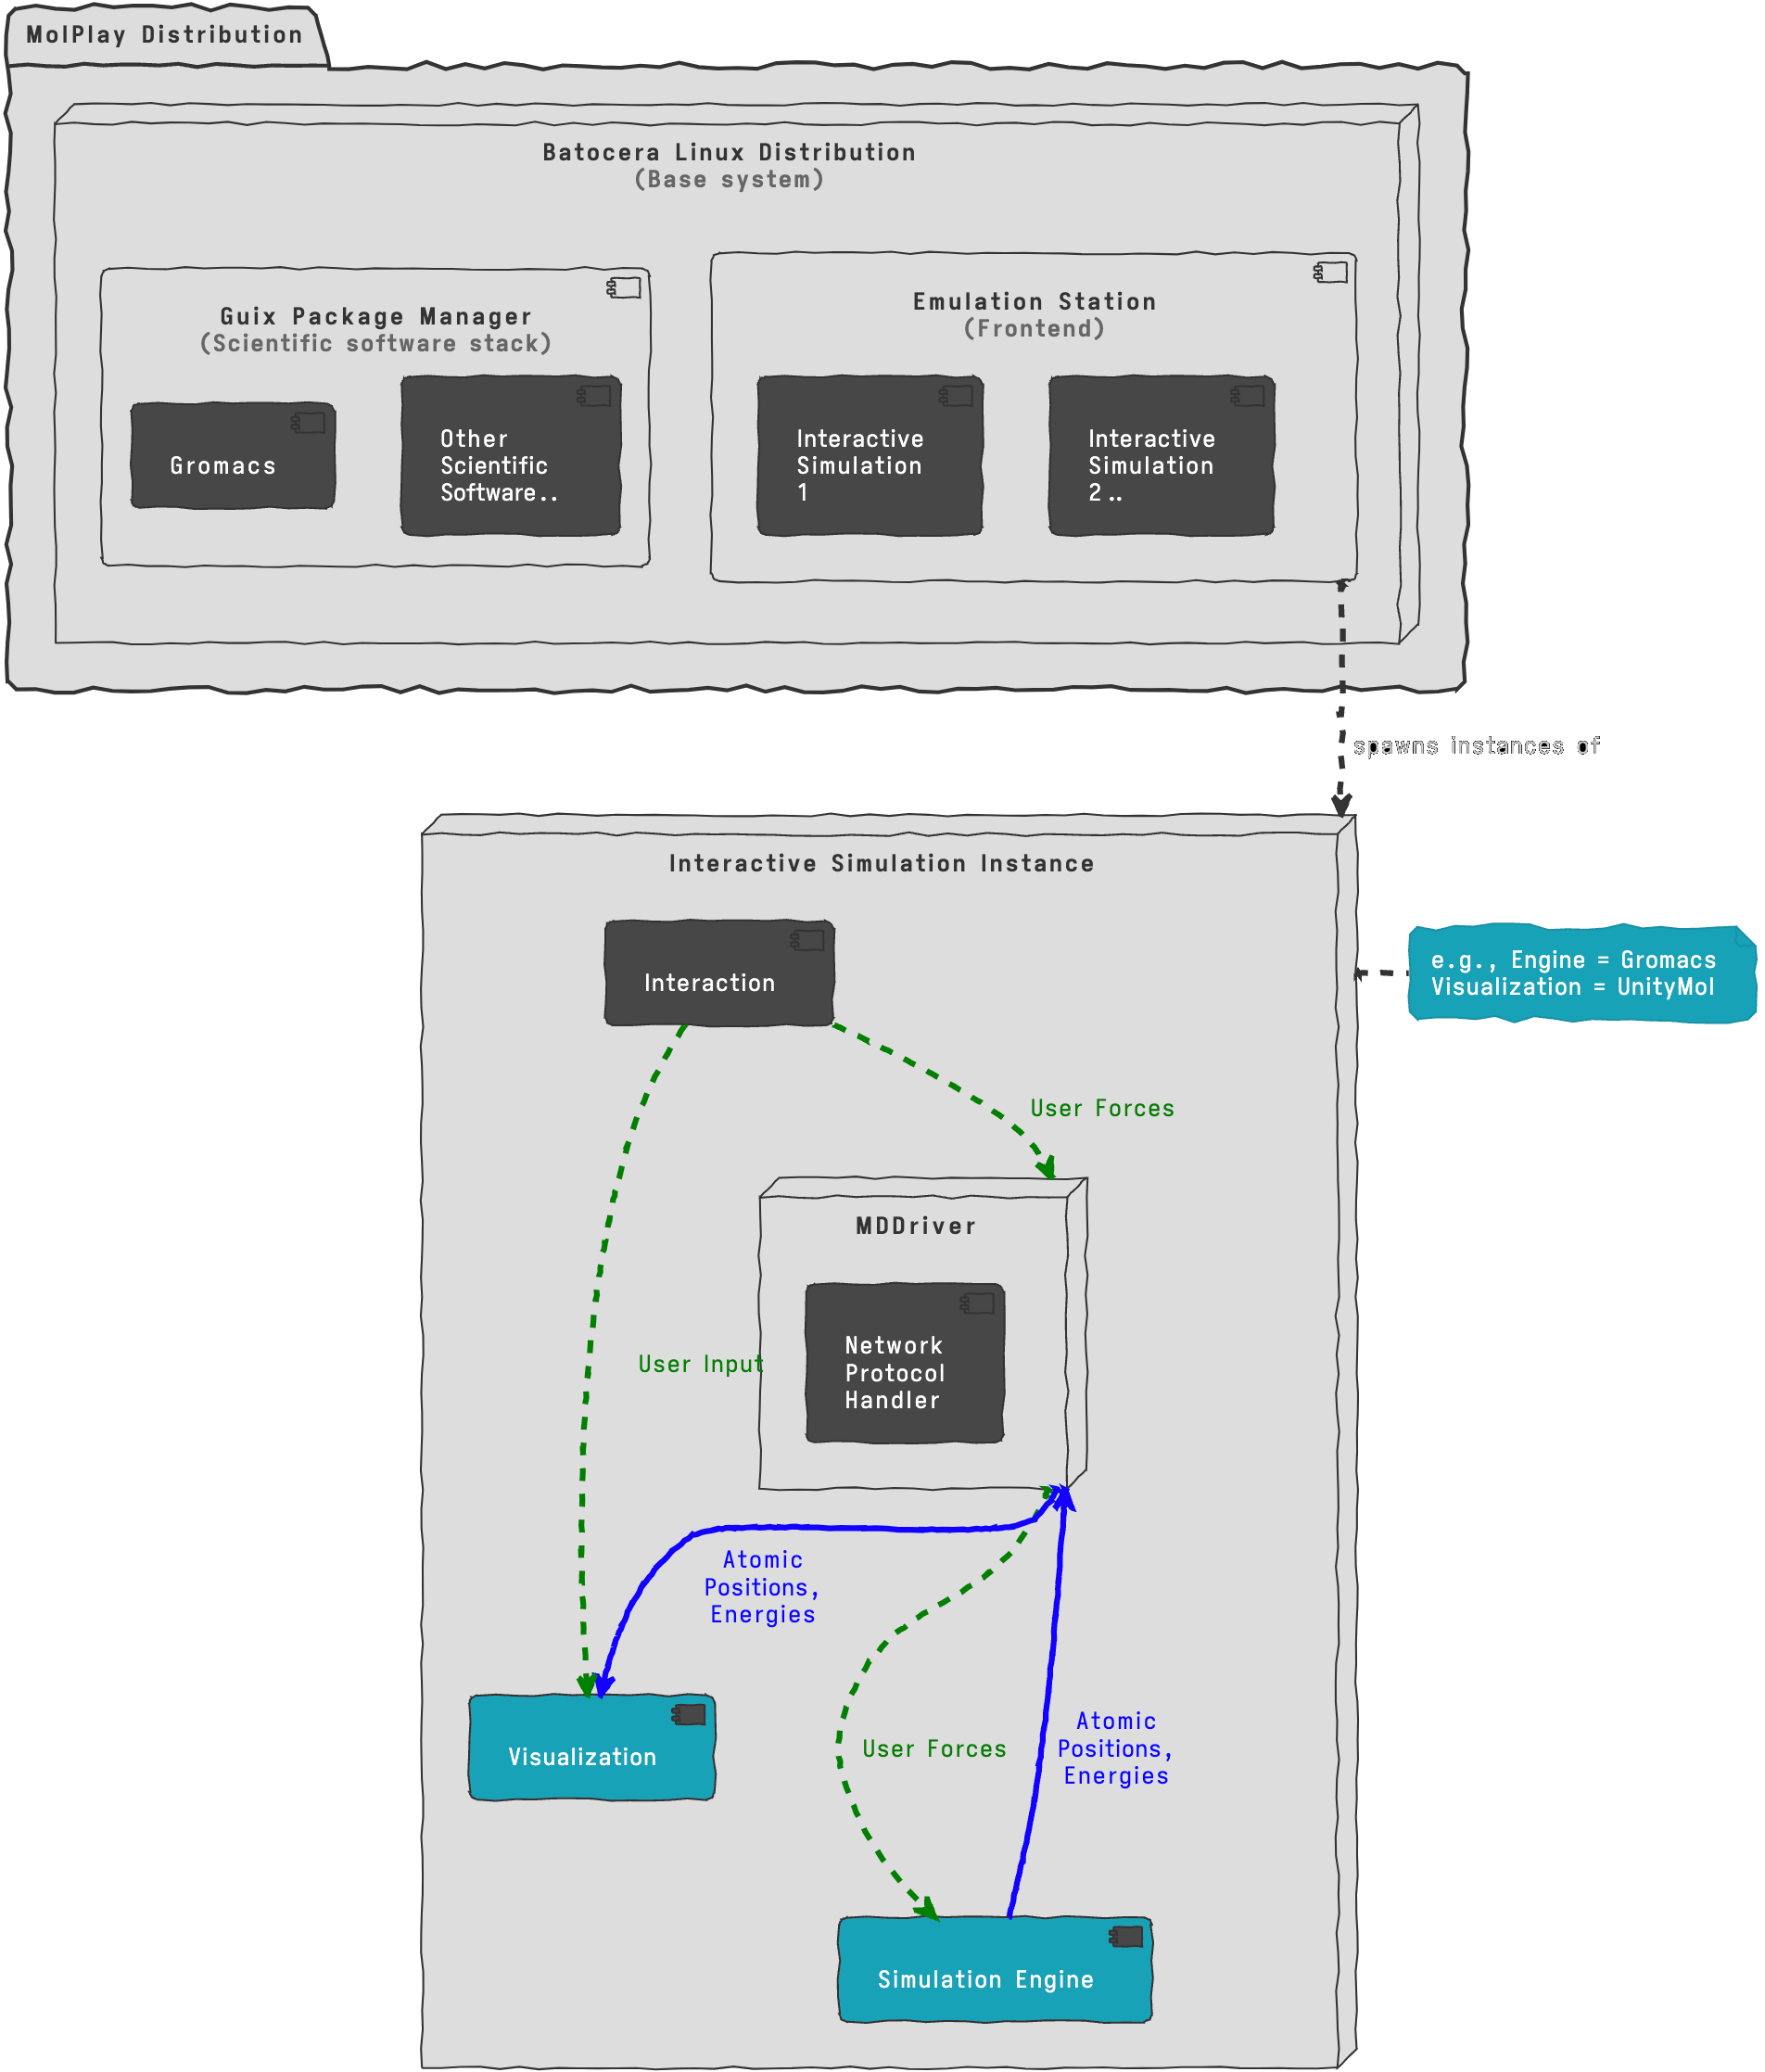
\includegraphics[width=.9\linewidth]{../img/molplay-scheme.png}
\caption{\label{fig:orgca1b7fb}An overview of MolPlay's architecture.}
\end{figure}

\begin{alertblock}{Components}
\begin{itemize}
\item \alert{Batocera Linux}: Lightweight base OS
\item \alert{Guix Package Manager}: Scientific software distribution
\item \alert{Emulation Station}: Intuitive menu interface
\item \alert{MDDriver Protocol}: Connects simulation components
\end{itemize}

\vspace*{1.8cm}
\end{alertblock}
\end{block}

\begin{block}{\emoji{microscope} Task Taxonomy}
We identified three \alert{main IMSA task categories}:
\begin{itemize}
\item \alert{Manipulate}: Model construction, deformation, force application
\item \alert{Explore}: Conformational sampling, rare event investigation
\item \alert{Analyze}: Real-time visualization, interaction scrutiny
\end{itemize}

\vspace{5mm}

These are depicted below:

\begin{figure}[htbp]
\centering
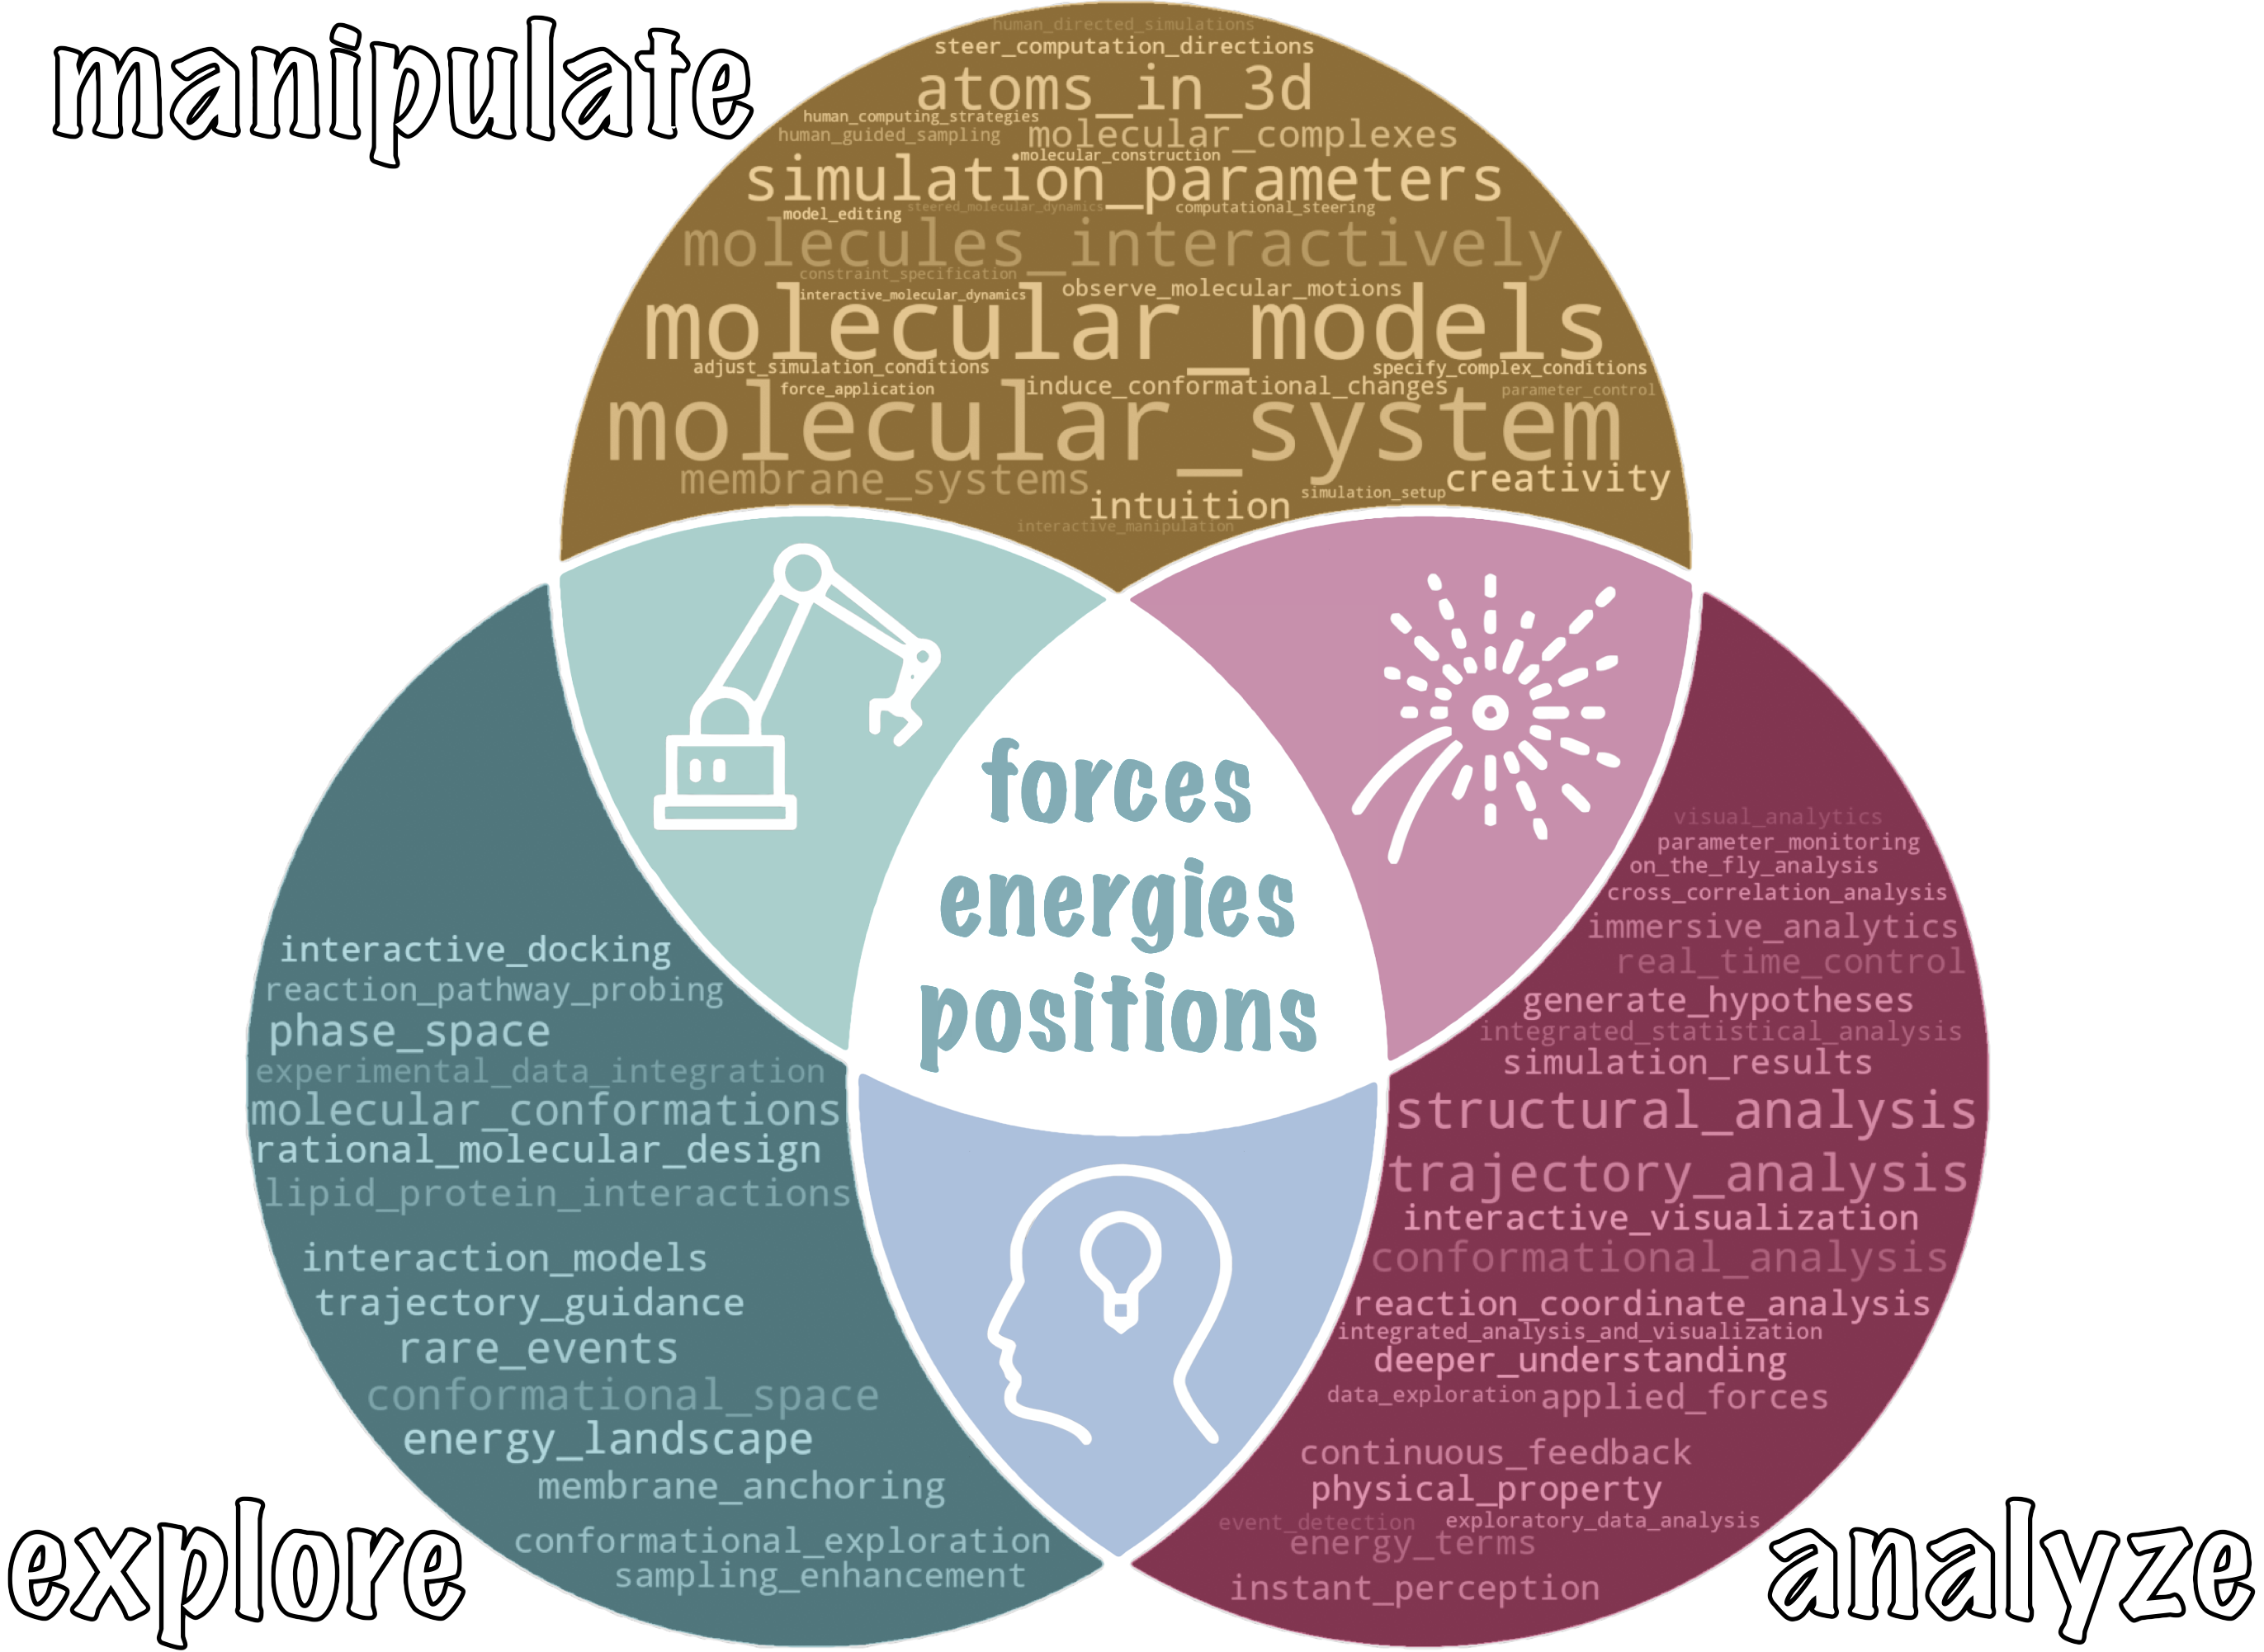
\includegraphics[width=.9\linewidth]{../img/tasks.png}
\caption{\label{fig:org7ea4a6d}Task categories for interactive approaches.}
\end{figure}
\end{block}
\end{column}

\begin{column}{0.27\columnwidth}
\begin{block}{\emoji{dna} Use Cases}
\begin{figure}[htbp]
\centering
\includegraphics[width=.9\linewidth]{../img/usecases.png}
\caption{\label{fig:org7833b0c}Four use cases for interactive simulations.}
\end{figure}

The examples above represent:
\begin{itemize}
\item \alert{A}: Preparing simulations - bending transmembrane helices
\item \alert{B}: Integrative modeling - ryanodine receptor reconstruction
\item \alert{C}: Mechanical properties - SNARE complex investigation
\item \alert{D}: Guided exploration - siderophore transport pathway
\end{itemize}

\vspace*{1.8cm}  
\end{block}

\begin{block}{\emoji{clapper} Ask for a Demo! \emoji{sparkles}}
\vspace*{1.0cm}  

\begin{center}

\includegraphics[width=.9\linewidth]{../img/demo.png}
\label{orgccbbb79}
\end{center}

\vspace*{1.8cm}  
\end{block}

\begin{block}{\emoji{video-game} User Experience}
\begin{figure}[htbp]
\centering
\includegraphics[width=.9\linewidth]{../img/menu.png}
\caption{\label{fig:org6cf400b}MolPlay's user interface is simple and user friendly.}
\end{figure}

\vspace{5mm}

Features:
\begin{itemize}
\item Simple boot from USB
\item Intuitive navigation
\item Built-in tutorials and documentation
\item Multiple levels of expertise
\end{itemize}

\vspace*{1.5cm}  
\end{block}

\begin{block}{\emoji{bullseye} Target Applications}
\begin{alertblock}{Education \& Outreach}
\begin{itemize}
\item Science fairs and museums
\item Classroom demonstrations
\item Hands-on learning experiences
\end{itemize}
\end{alertblock}

\begin{alertblock}{Research}
\begin{itemize}
\item Hypothesis validation
\item Preliminary investigations
\item Collaborative analysis
\end{itemize}

\vspace*{1.8cm}  
\end{alertblock}
\end{block}

\begin{block}{\emoji{game-die} Featured Simulation Engine \autocites{biospringurl}[][]{hal-05039981}}
\vspace*{1.0cm}  

\begin{center}
\includegraphics[width=.9\linewidth]{../img/biospring.png}
\label{orgd920e16}
\end{center}
\end{block}
\end{column}



\begin{column}{0.27\columnwidth}
\begin{block}{\emoji{eyes} Visual Analysis}
\begin{figure}[htbp]
\centering
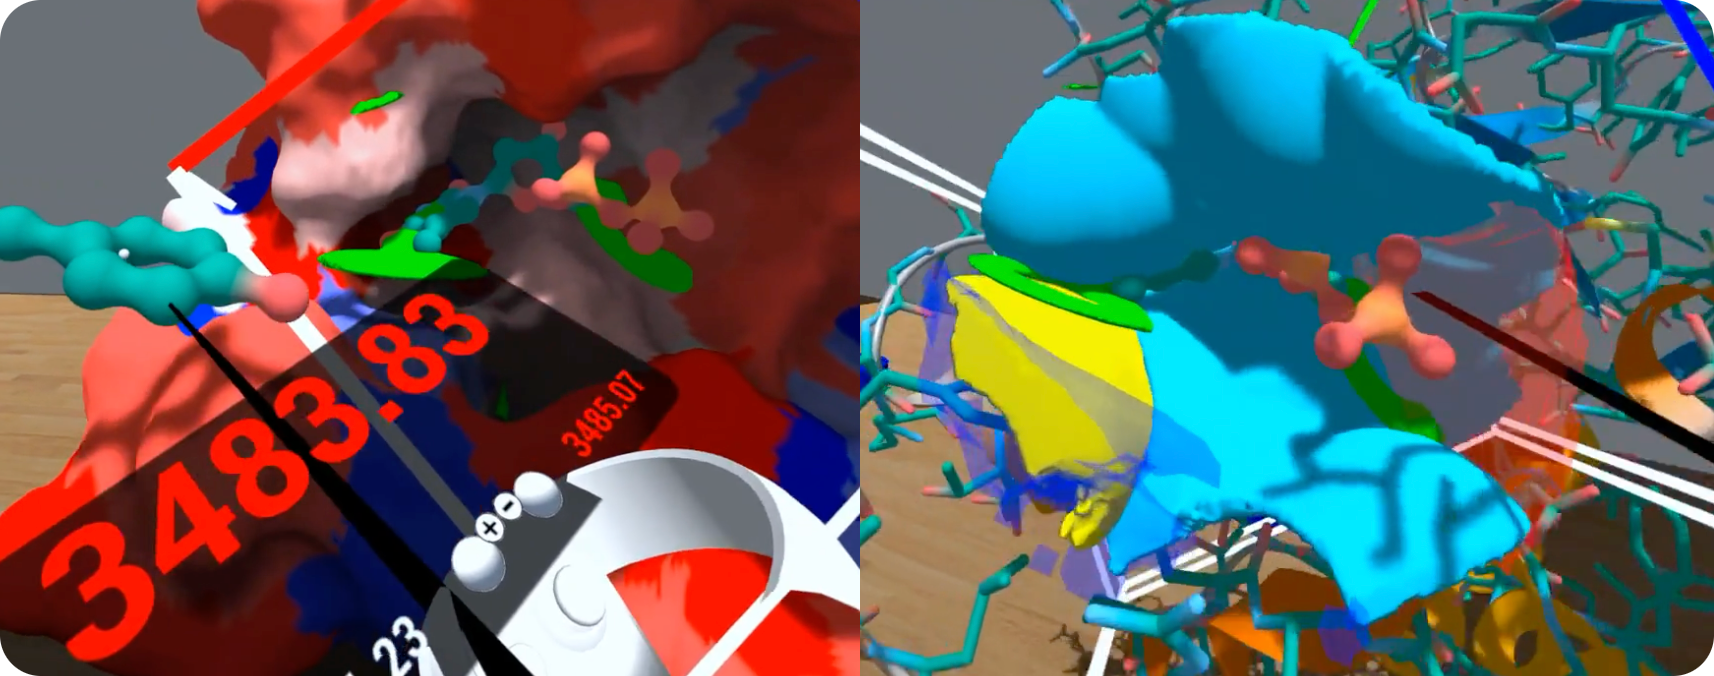
\includegraphics[width=.9\linewidth]{../img/smiffer.png}
\caption{\label{fig:orgaea4df2}Visual analysis of statistical molecular interaction fields \autocites{smifferurl}[][]{smifferpreprint}.}
\end{figure}

\vspace*{1.8cm}  
\end{block}

\begin{block}{\emoji{chart-increasing} Impact \& Future}
\begin{itemize}
\item \alert{Tested} at international workshop (\textasciitilde{}30 participants)
\item \alert{Positive feedback} from diverse user groups
\item \alert{Expandable} catalog of examples
\item \alert{Modular design} for future integrations
\end{itemize}

\vspace*{1.8cm}  
\end{block}

\begin{block}{\emoji{interrobang} Conclusions}
MolPlay bridges the gap between advanced IMSA techniques and accessible education/research tools. By consolidating expertise into a portable platform, it promotes broader adoption of interactive molecular simulations across disciplines.

\vspace*{1.8cm}  
\end{block}

\begin{block}{\emoji{performing-arts} Acknowledgments}
M.B. thanks past (Sébastien Doutreligne, André Lanrezac, Xavier
Martinez, Joao Rodriguez, Alex Tek) and present (Olivier Delalande,
Nicolas Férey, Benoist Laurent, Hubert Santuz) collaborators who were
essential in laying the foundations for the work described on this
poster.

\vspace*{1.8cm}  
\end{block}

\begin{block}{\emoji{euro-banknote} Funding}
This research was funded by the “Initiative d’Excellence” program from
the French State, grants “DYNAMO,” ANR-11-LABX-0011, and “CACSICE,”
ANR-11-EQPX-0008. I thank ANR for support of grants “PIRATE,”
ANR-21-CE45-0014 and “MINOMICS,” ANR- 19-CE45-0017. Many thanks to
Sesame Ile-de-France for co-funding the display wall used for testing
some of the interactive use cases described on the poster.

\vspace*{1.8cm}  
\end{block}

\begin{block}{\emoji{bookmark-tabs} References and links}
\printbibliography

\vspace*{1.8cm}  
\end{block}

\begin{block}{\emoji{telephone-receiver} Contact}

\includegraphics[width=0.035\linewidth]{../img/atsign.png}    Email: \href{mailto:baaden@smplinux.de}{baaden@smplinux.de}
\vspace*{0.3cm}


\includegraphics[width=0.035\linewidth]{../img/website.png}    Website: \href{https://www.baaden.ibpc.fr}{www.baaden.ibpc.fr}
\vspace*{0.3cm}


\includegraphics[width=0.035\linewidth]{../img/linkedin.png}    LinkedIn: \href{https://linkedin.com/in/baaden}{baaden}
\vspace*{0.3cm}


\includegraphics[width=0.035\linewidth]{../img/mastodon.png}    Mastodon: \href{https://mastodon.social/@baam93}{@baam93@mastodon.social}
\vspace*{0.3cm}


\includegraphics[width=0.035\linewidth]{../img/bluesky.png}    Bluesky: \href{https://bsky.app/profile/baam93.bsky.social}{@baam93.bsky.social}
\vspace*{0.3cm}


\includegraphics[width=0.035\linewidth]{../img/twitterx.png}    Twitter/X: \href{https://x.com/baam93}{@baam93}
\vspace*{1.8cm}  

% \begin{flushright}
% 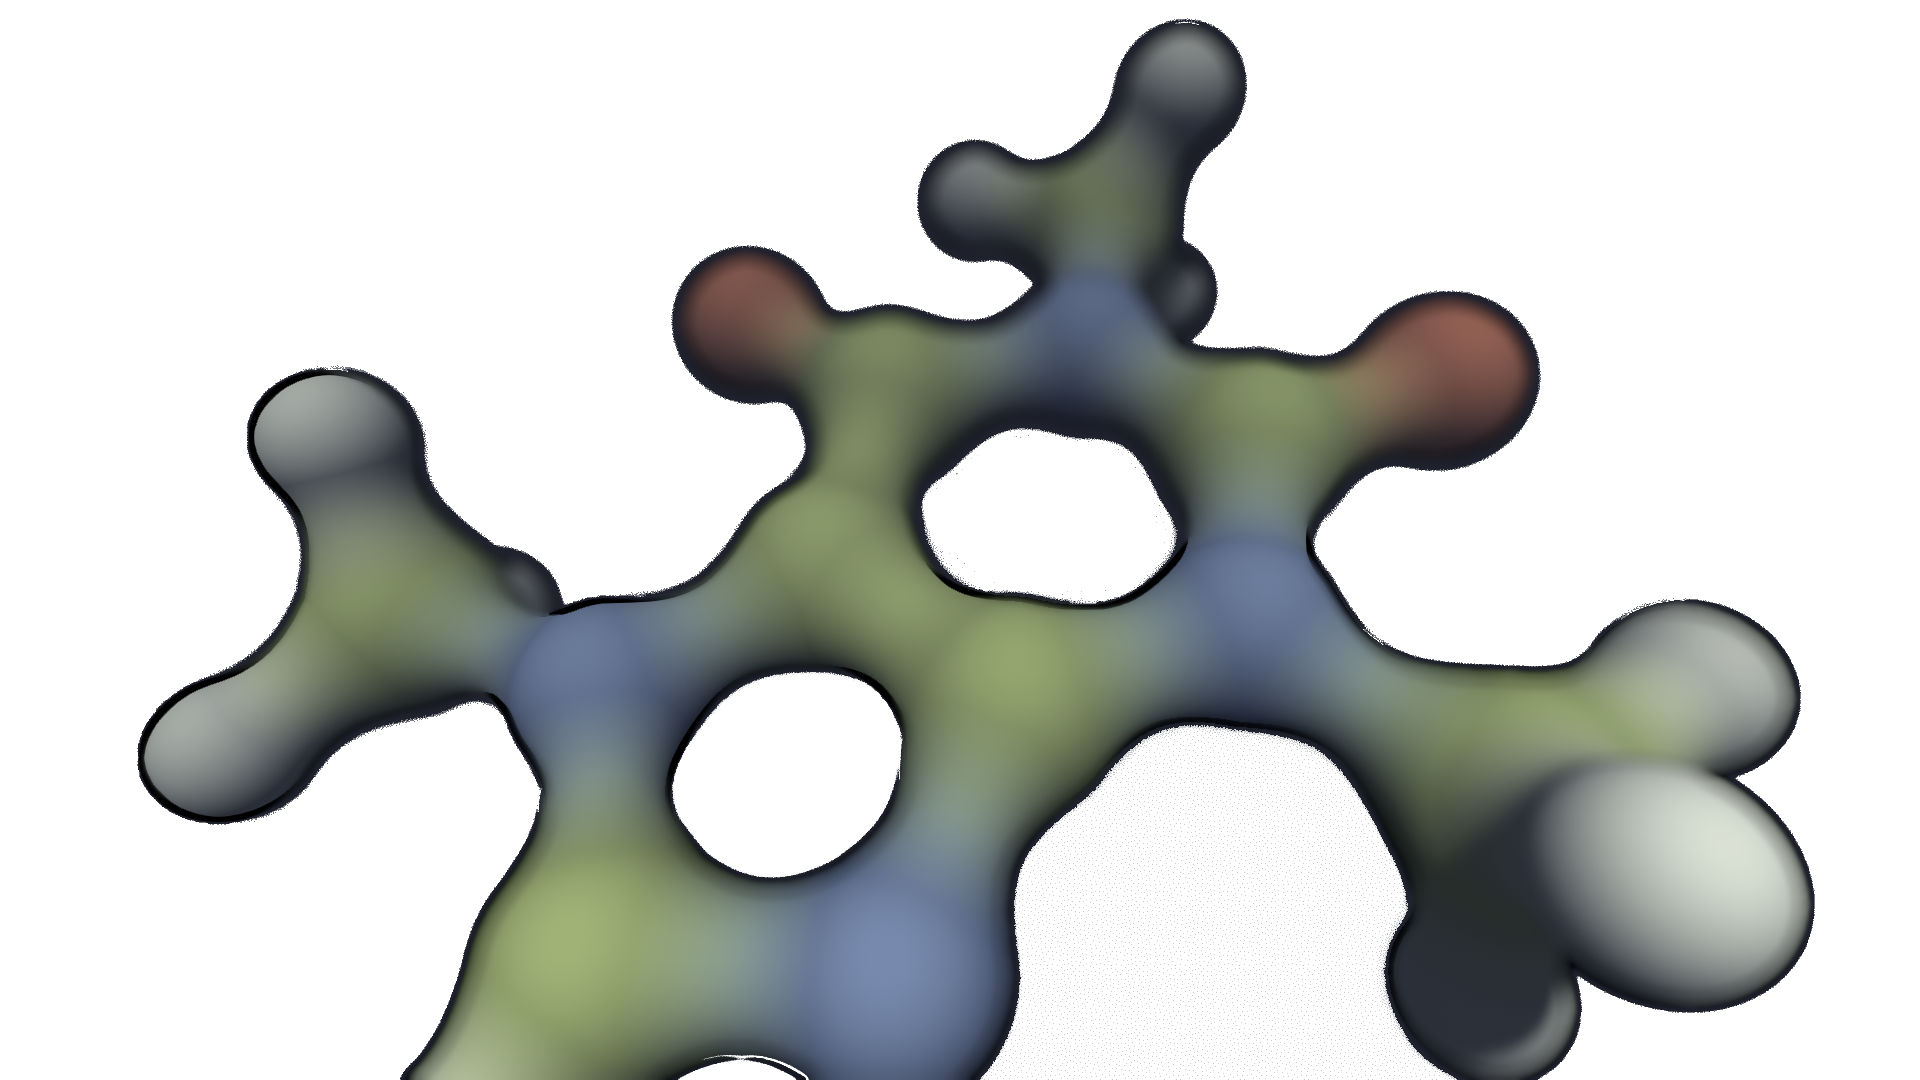
\includegraphics[width=1.5\linewidth]{../img/caffeine.png}
% \end{flushright}
\begin{textblock*}{5cm}(55.0cm,102cm) % Width x (X,Y) from top-left
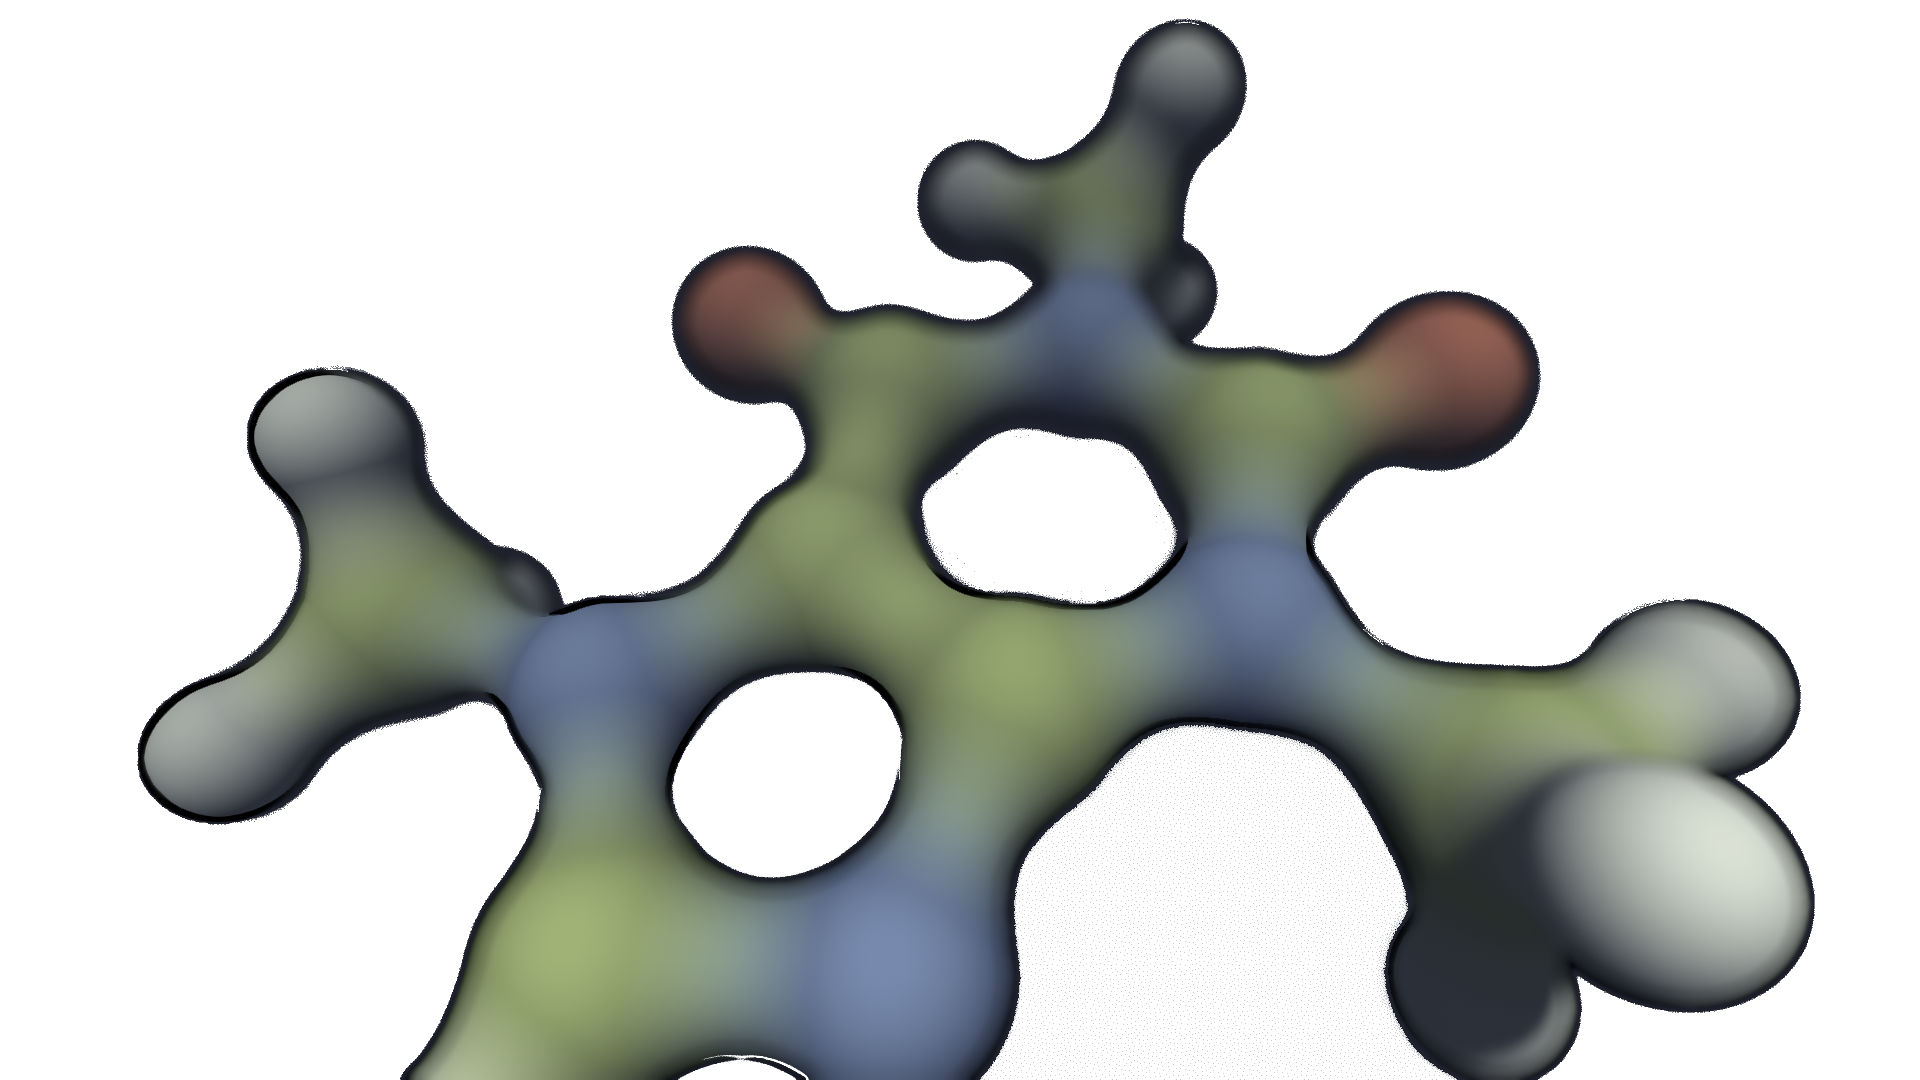
\includegraphics[width=6.0\linewidth]{../img/caffeine.png}
\end{textblock*}

\begin{textblock*}{5cm}(57cm,4cm) % Width x (X,Y) from top-left
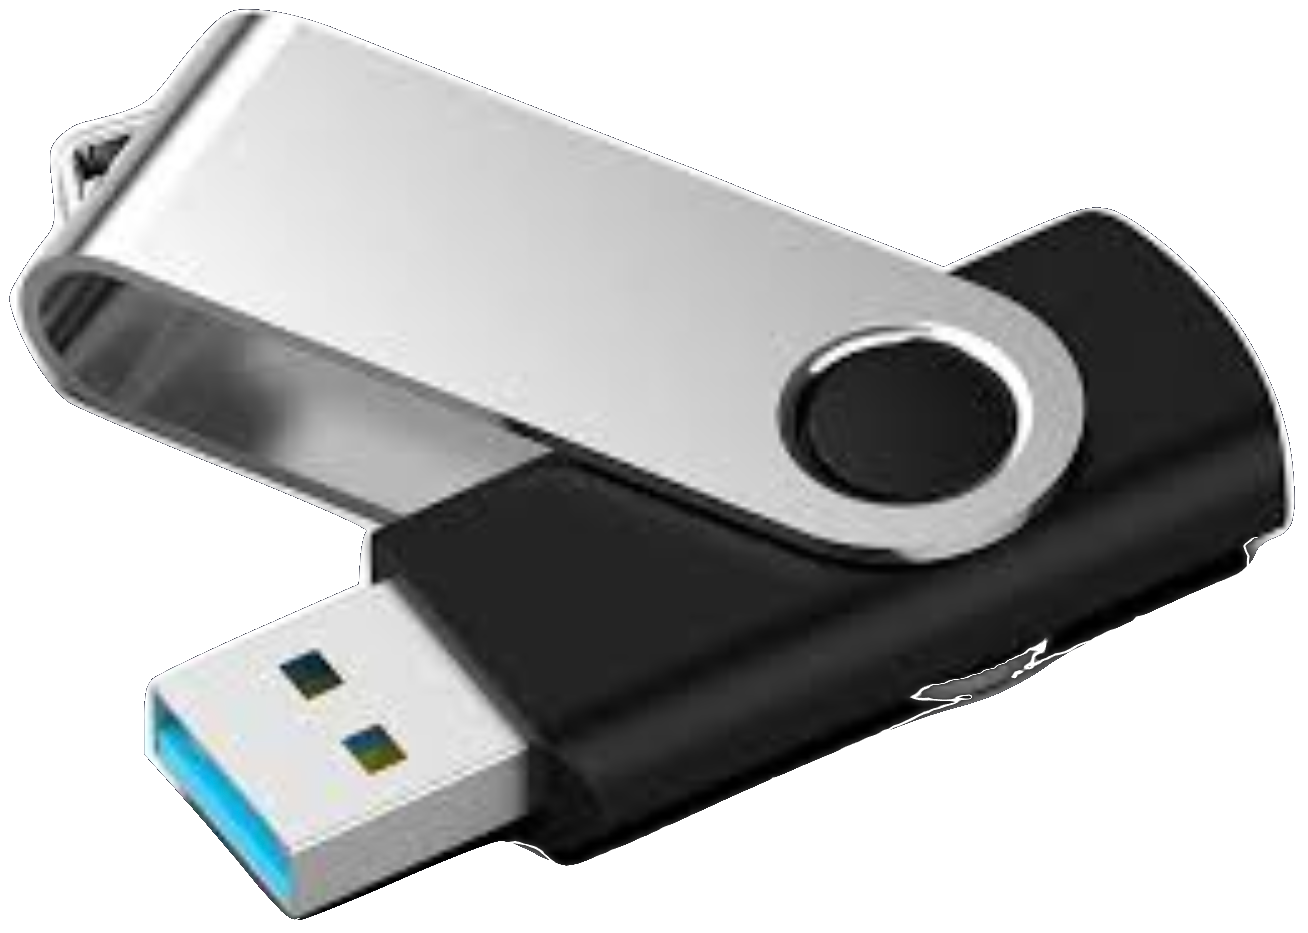
\includegraphics[width=2.0\linewidth]{../img/cleusb.png}
\end{textblock*}
\end{block}
\end{column}
\end{columns}
\end{frame}
\end{document}
